% This file should be replaced with your file with an thesis content.
%=========================================================================
% Authors: Michal Bidlo, Bohuslav Křena, Jaroslav Dytrych, Petr Veigend and Adam Herout 2019

% For compilation piecewise (see projekt.tex), it is necessary to uncomment it and change
% \documentclass[../projekt.tex]{subfiles}
% \begin{document}

\chapter{Introduction}
This chapter summarizes the motivation and objectives of this thesis, the solution taken to achieve the objectives, and the results of the thesis. In the last section, the structure of the thesis is presented.

\section{Motivation and Objectives}
This work was initiated by Honeywell International Inc. \cite{honeywell}, which currently uses IBM Doors as a solution for requirement management. The company is exploring the option and considering switching to a new solution -- Jira R4J. Honeywell currently provides its clients access to requirements stored in IBM Doors via the OSLC interface for Requirement Management Specification, which comes with IBM Doors. The company is interested in providing the same access to requirements stored in Jira R4J. The goal of this thesis is to explore and create a solution that will allow Honeywell to provide its clients with access to requirements stored in Jira R4J via the OSLC interface for Requirement Management Specification.

\section{Solution}
There are two ways to add OSLC support to a web application, either as an add-on or a standalone web application. After careful consideration, a decision was made to create the adaptor as a standalone web application. The main reason for this decision was to reduce the coupling between the web application and the OSLC interface, which allows for easier maintenance and development, as well as the possibility of using the OSLC adaptor with other web applications, besides Jira R4J, in the future. 

During the initial design phase, it was also decided to split the adaptor into two separate adaptors. One for Jira, responsible for the main functionality specified by the Requirement Management Specification, and one for R4J, providing additional functionality, such as the ability to create folders and link requirements to folders. This decision was made in order to explore the possibility of not needing to use the R4J plugin at all and instead using Jira directly. It also leads to the final solution being generic and less coupled to a specific web application, allowing for easier enhancement or replacement of the underlying web application in the future.

Both adaptors were created using Eclipse Lyo, a project containing SDKs and other utilities used for easier development of OSLC applications. Lyo Designer was used to create the Domain and Toolchain models, which represent the data and capabilities of both adaptors. These models were then fed to Code Generator to generate the code skeletons, compliant with the OSLC specification, for the adaptors. The generated skeletons were then filled with the actual code, implementing the functionality of the adaptors and extended with additional functionality, such as OAuth2 authentication.

\section{Results}
Both adaptors were created as standalone REST-based Java web applications built on the Maven framework. During the development, a collection of HTTP requests was created in Postman, detailing the example usage of created adaptors. The functionality of both adaptors was verified by end-to-end testing, utilizing the Postman Test utility. For further verification of the base capability of Requirement Management Specification, implemented in Jira adaptor, a basic Python client was developed, providing the option to download and upload all of the requirements, in the specified project, in the ReqIF format.

The mapping of the data provided by Jira and R4J API to the OSLC format was done as generically as possible to accommodate all possible use cases, which differ significantly between different companies. During the development, some issues and missing functionality were discovered in the R4J API, resulting in the non-optimal implementation of some of the functionality of the R4J adaptor.

The utilities and SDKs provided by Eclipse Lyo were very useful in the development and design stages of the adaptors, greatly reducing the time needed to adopt the OSLC standard. However, the documentation and examples provided by the Lyo project were outdated and not detailed enough, also lacking some deeper explanation of important concepts. The contents of the Requirement Management Specification were also not documented sufficiently, compared to, for example, the Automation Domain Specification, resulting in difficulties in the comprehension of the specification.

\section{Structure of the Thesis}
%\todo{Gramar check}
%\todo{Style document}
\todo{Write after thesis structure is finalized}

%=========================================================================

\chapter{Background}
This chapter briefly covers the basics of requirements management and its fundamental concepts, as well as a basic overview of Jira Software and Requirements for Jira plugin. Information provided in this overview is important for understanding the requirements and needs of the adaptor.

\section{Requirements Management}
The aim of requirement management is the verification of the accomplishment of the project's goals and objectives. The process is divided into several successive stages, the most essential being analysis, documentation, tracing, and change control. The purpose of this process is to track the requirements and their status, identify inconsistencies and provide an overview of the project progress to concerned stakeholders \cite{requirements_management}.

One of the most important parts of requirement management is \emph{traceability}. It is the ability to track and assess the state of the requirement and its changes during the development lifecycle, providing an audit trail, usually used for reporting to stakeholders. Traceability can be achieved by linking requirements to other requirements, test cases, or build stories.

\subsection*{Requirements}
\label{sec:requirements}
Requirements are the foundation for determining the needs of system stakeholders and the system itself. They represent a condition or capability
that must be met by a system or product \cite{IEEE_24765-2017}.

They can be divided into two main categories, \emph{functional} and \emph{non-functional} requirements. Functional requirements describe the system behavior or product features (e.g., the system will send an email with a forgotten password prompt when requested by the user), while non-functional requirements usually specify the system's performance or product properties (e.g., a task has to be completed under 200 ms).

\section{Requirement Management Systems}
Requirement Management System is a software tool used for the management of project requirements during the development lifecycle. Currently, there are several different requirement management systems developed by competing companies available on the market. Some of the most popular ones are IBM Doors and Jira Software with Requirements for Jira plugin. A high-level overview of these options is provided in the following sections, as they are important in the context of this thesis.

\subsection*{IBM Doors}
IBM Doors \cite{ibm_doors} is a requirement management system developed by IBM \cite{ibm}. It is a complex tool designed to handle large projects with many requirements and stakeholders. The tool is commonly used in the aerospace, defense, and automotive industries. It provides a wide set of features to aid in the requirement management processes, such as requirement traceability, collaboration, and ease of integration with other IBM tools. It is also designed in a way to help companies comply with industry standards and regulations for requirement management and project development. All of the previously mentioned features are available through the web user interface, REST API as well as native OSLC interface.

\subsection*{Jira Software and Requirements for Jira}
\textbf{Jira Software} \cite{jira} is an issue-tracking and project management tool developed by Atlassian \cite{atlassian}. Compared to IBM Doors, it provides a more user-friendly interface and is more flexible, as its functionality spans across many different areas, such as project management, test management, and bug tracking. It also allows the end customers to extend the capabilities of their Jira instance by adding plugins developed by Atlassian or third-party developers, augmenting the original functionality, or adding completely new features. The contents of Jira and its functionality are accessible through the web user interface or REST API \cite{jira_api} with BASIC or OAuth2 authentication, further described in chapter \ref{chapter:authentication}. It does not provide a native OSLC interface, but the support for OSLC can be added by installing a third-party plugin (e.g., OSLC Connector for Jira \cite{oslc_connector_for_jira} for Change Management Specification).

\textbf{Requirements for Jira} (R4J) \cite{requirements_for_jira} is a native Jira plugin extending the capabilities of Jira by adding support for requirements management by making use of Jira issues. It provides the ability to manage requirements by creating a folder structure, enabling importing and exporting in the reqIF format, enabling traceability, by utilizing the Jira link functionality, and adding the option to export these links into a comprehensive traceability matrix. All of these features are available both from the Jira web user interface as well as from the R4J REST API \cite{r4j_api}. Because the requirement management system provided by R4J is a part of Jira, it allows for better traceability, as the requirements can not only be linked to other requirements but also to other Jira issue types, such as bugs, stories, test cases, and many more.

\section{Requirements Interchange Format}
Requirements Interchange Format (ReqIF) \cite{reqif_standard} is an XML-based format used for transferring and sharing requirements between requirement management systems or other tools. The format defines a standardized way to describe requirements, their attributes and properties, relations between requirements, and a hierarchical structure, in which the requirements are contained. Each object, type, attribute, and relation contains a unique identifier by which it can be referenced from other objects.

The document is divided into two parts, \texttt{THE-HEADER}, containing metadata information about the requirement collection, and \texttt{CORE-CONTENT}, which is then further split into five sections, each containing different information about the requirements:

\begin{itemize}
  \item \texttt{DATATYPES} -- definitions of datatypes used in the document
  \item \texttt{SPEC-TYPES} -- definitions of types of requirements, its attributes and relations, the data type of the attribute is defined by a reference to a definition in \texttt{DATATYPES}
  \item \texttt{SPEC-OBJECTS} -- a collection of requirements and its properties, described in a format specified in \texttt{SPEC-TYPES}
  \item \texttt{SPEC-RELATIONS} -- a collection of relations between requirements, described in a format specified in \texttt{SPEC-TYPES}
  \item \texttt{SPECIFICATIONS} -- requirements hierarchical tree structure
\end{itemize}

%=========================================================================

\chapter{OSLC -- Open Services for Lifecycle Collaboration}
This chapter provides a brief overview of the OSLC (Open Services for Lifecycle Collaboration) \cite{oslc}, its fundamental technologies, and the Core and Requirement Management specifications, which are used in this thesis.

\section{Overview}
OSLC \cite{oslc} is an OASIS Open Project \cite{oasis_open} responsible for developing a set of open specifications, which are used for easier integration of software tools. A more detailed overview of the OSLC project can be found in the \emph{OSLC Primer} \cite{oslc_primer}.

The initiation of the OSLC project was driven by the increasing number of software tools, which are used in the software development lifecycle. These tools are usually developed by different organizations, which leads to the problem of difficult tool integration. In the past, this was solved by developing specific translators and adaptors for each tool, which was a time-consuming and expensive process. OSLC was created to solve this problem, by creating a set of open specifications to integrate the resources managed by the software tools into the web of data.

OSLC offers two different methods of data integration -- \emph{Linking data via HTTP} and \emph{Linking Data via HTML User Interface} \cite{oslc_primary_integration_techniques}.


\subsection*{Linking data via HTTP}
Linking of the data via HTTP is based on OSLC-defined common tool protocol for accessing, creating, updating, and deleting resources. The protocol is based on internet technologies and standards, such as REST, RDF, and Linked Data, described in section \ref{sec:oslc_fundamental_technologies}. It allows any other tool, that implements the same specification, to access any of the managed resources. Linking of the data is done by referencing resources by HTTP URIs in the representations of other data.

\subsection*{Linking Data via HTML User Interface}
\label {sec:oslc_linking_data_via_html_user_interface}
OSLC protocol can be used to link data via HTML user interface as well, making use of the REST code on demand constraint. This allows the client to access and display fragments of an existing user interface, provided by the tool, without the need to implement the user interface itself. This delegated user interface then enables the client to access the resources managed by the tool.

\section{Fundamental Technologies}
\label {sec:oslc_fundamental_technologies}
OSLC is built on top of several fundamental technologies. This section lists these technologies and introduces briefly each of them.

\subsection*{REST}
REST (REpresentational State Transfer) \cite{rest} is a web software architecture style, describing a set of constraints and properties, which should be followed in communication between computer systems, most commonly between client and server. In REST architecture, the server is responsible for exposing a common interface, which allows the client to access resources by using standard HTTP methods. Each resource the server provides has a unique identifier, that allows the resource to be identified unambiguously and completely. When requested, the server responds with a representation of the resource. The client can then use this resource to create new resources and update or delete existing resources. The communication between the server and the client is stateless, meaning every request the server receives can be fully understood in isolation, without the context of previous requests. The most common HTTP methods used in REST are \texttt{POST}, \texttt{GET}, \texttt{PUT}, and \texttt{DELETE}, which correspond to the CRUD operations (Create, Read, Update, and Delete).

\subsection*{RDF}
RDF (Resource Description Framework) \cite{rdf} is a W3C (World Wide Web Consortium) \cite{w3c} standard for representing data on the web. It describes resources in the form of a directed graph, where information about each element is represented as a triplet. Triplets are statements about the resource composed of subject, predicate, and object. The subject describes the resource, and the predicate specifies its properties and relationships, between the subject and the object. Most widely used RDF serialization formats are Turtle \cite{turtle}, RDF/XML, and RDF/JSON.

\begin{figure}[hbt]
  \centering
  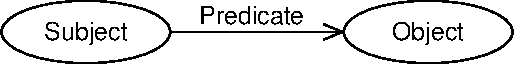
\includegraphics[width=.6 \linewidth]{figures/rdf-graph.pdf}
  \caption{RDF Graph Triplet (source: \cite{rdf_primer})}
  \label{fig:rdf_graph_triplet}
\end{figure}

\subsection*{Linked Data}
Linked Data \cite{linked_data} are structured data containing references to other data. This enables computers to query and interpret the data, allowing the internet to become one big database. The main principles of Linked Data are \cite{linked_data_design_issues}:
\begin{enumerate}
  \item URIs \cite{uri_rfc} are used as names to identify things
  \item People can lookup things using HTTTP URIs
  \item Information returned as a result of the search are provided in an open standard format (for example RDF)
  \item Returned information contain more URIs, enabling discovery of other things
\end{enumerate}

\section{OSLC Specifications}
OSLC defines a set of open specifications for integrating software tools. OSLC consists of multiple working groups, which are each responsible for the development of a specific specification. There are two types of specifications -- \emph{Core} and \emph{Domain}. The Core specification provides a basis for the Domain specifications, which are then focused on a specific field, for example, Requirement Management, Change Management, Configuration Management, etc. This section provides a summary of the OSLC Core and Requirement Management specifications, which are used in this thesis.

\subsection{OSLC Core Specification}
\label{sec:oslc_core_specification}
At the time of writing this thesis, the current version of OSLC Core Specification \cite{oslc_core_specification} is 3.0. The OSLC Core Specification defines a set of common principles, capabilities, and restrictions, which should be common across all OSLC Domain Specifications. Specific OSLC Domain Specification will then describe which of these capabilities are required or optional for conformance with the specification. It also introduces several resource types and properties with the namespace \url{http://open-services.net/ns/core\#} and prefix \emph{oslc}. In the following sections, a basic overview of the core concepts is provided.

\begin{figure}[hbt]
  \centering
  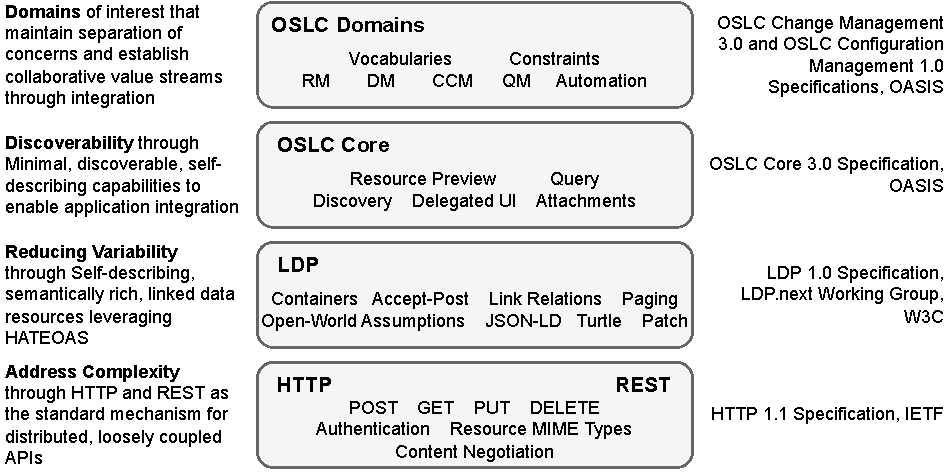
\includegraphics[width= \linewidth]{figures/OSLC-core.pdf}
  \caption{OSLC Core 3.0 architecture (source: \cite{oslc_core_specification}, remade)}
  \label{fig:oslc_core_architecture}
\end{figure}

\subsection*{Resource Shape}
OSLC works with resources, which are uniquely identified by a URI \cite{uri_rfc}, and are represented by RDF triples. Resource Shape \cite{oslc_core_resource_shape} is a resource of type \texttt{oslc:ResourceShape}, that describes the contents and constraints of other resources.

\begin{figure}[hbt]
  \centering
  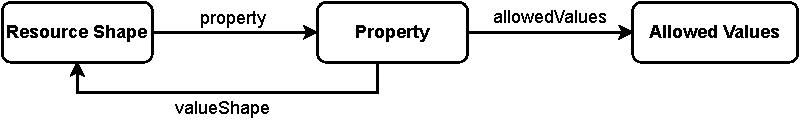
\includegraphics[width=.8 \linewidth]{figures/resource-shape.pdf}
  \caption{Resource Shape (source: \cite{oslc_core_resource_shape}, remade)}
  \label{fig:resource_shape}
\end{figure}

Each Resource Shape has a defined set of Properties, of type \texttt{oslc:Property}, which specifies the value type and cardinality of the property. The value type of the property can be either a reference to another Resource Shape, or a basic data type. The cardinality of the Property specifies if the Property is required, optional, or can be present multiple times. OSLC Core Specification defines these basic data types: \texttt{XMLLiteral}, \texttt{boolean}, \texttt{dateTime}, \texttt{decimal}, \texttt{double}, \texttt{float}, \texttt{integer}, \texttt{string}, and \texttt{langString}.

\subsection*{Discovery}
For the reasons of flexibility and to reduce coupling, the OSLC Core Specification does not specify unequivocally which capabilities the server has to provide. Instead, it offers a mechanism for the incremental discovery of services and capabilities the target server has implemented.

\begin{figure}[hbt]
  \centering
  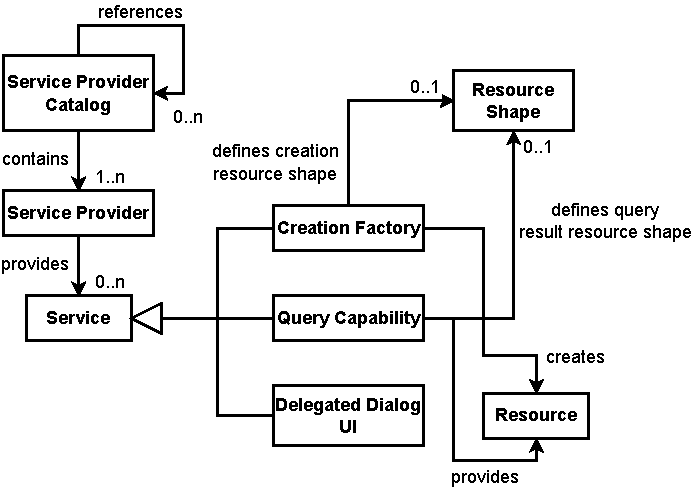
\includegraphics[width=.8 \linewidth]{figures/oslc-discovery.pdf}
  \caption{OSLC Discovery diagram (source: \cite{oslc_core_discovery}, remade)}
  \label{fig:oslc_discovery}
\end{figure}

The server always has to specify the starting point of discovery, which is the \emph{Service Provider Catalog}. The Service Provider Catalog is a resource containing a list of available \emph{Service Providers}, which then contains all of the available \emph{Services}. From there, the client is able to find the URIs for \emph{Creation Factories}, \emph{Dialogs}, and \emph{Query services}. For additional information about the Discovery mechanism can be found in the Discovery section of the OSLC Core Specification \cite{oslc_core_discovery}.


\subsection*{Basic Capabilities}
OSLC Core Specification defines basic CRUD (Create, Read, Update, Delete) operations for resources. However, the decision about which of these operations are required or optional for which resource is specified in each of the OSLC Domain Specifications. Read, Update, and Delete operations are performed by their respective HTTP request method to the URI of the target resource. Create operation is performed by a \texttt{POST} operation to the Creation Factory URI for a specific resource.

\subsection*{Delegated UI}
OSLC Core Specification introduces Delegated UI \cite{oslc_core_delegated_ui} for resource creation -- \emph{Creation Dialog}, and resource selection -- \emph{Selection Dialog}. Both of these dialogs are examples of linking of the data via HTML mentioned in \ref{sec:oslc_linking_data_via_html_user_interface}. Dialogs are returned as a combination of HTML \texttt{iframe} and JavaScript code. The decision about which of these dialogs are required or optional is again left up to the OSLC Domain Specification.

\subsection*{Query Capability}
As the OSLC server manages a large number of resources, it has to provide a way for clients to search and filter these resources. OSLC Core Specification specifies a mechanism for this, called OSLC Query \cite{oslc_core_query}. OSLC Query allows clients to look up a set of resources by performing a \texttt{GET} or \texttt{POST} request on an \texttt{oslc:queryBase} URI. It offers two separate capabilities, a full-text search, identified by the \texttt{oslc.searchTerms} parameter, and a query search for resources containing specific properties and values, identified by \texttt{oslc.where} parameter. Each query search must consist of at least one property, comparison operator, and value. The result of the search is returned as a resource of type \texttt{oslc:QueryResult}, which contains a list of references to the resources found (example of \texttt{oslc:QueryResult} can be found seen in Listing \ref{lst:oslc_query_result}).

\begin{lstlisting}[
  language=XML, label={lst:oslc_query_result}, float=hbt,
  caption={OSLC Query Result example}
]
<?xml version="1.0" encoding="UTF-8"?>
<rdf:RDF
  xmlns:rdf="http://www.w3.org/1999/02/22-rdf-syntax-ns#"
  xmlns:dcterms="http://purl.org/dc/terms/"
  xmlns:oslc_data="http://open-services.net/ns/servicemanagement/1.0/"
  xmlns:oslc="http://open-services.net/ns/core#"
  xmlns:oslc_rm="http://open-services.net/ns/rm#"
  xmlns:rdfs="http://www.w3.org/2000/01/rdf-schema#"
  xmlns:foaf="http://xmlns.com/foaf/0.1/">
  <oslc:ResponseInfo rdf:about="...">
    <oslc:totalCount rdf:datatype="http://www.w3.org/2001/XMLSchema#int"
  >2</oslc:totalCount>
  </oslc:ResponseInfo>
  <rdf:Description rdf:about=".../queryRequirement">
    <rdfs:member>
      <oslc_rm:Requirement rdf:about="...">
        ...
      </oslc_rm:Requirement>
    </rdfs:member>
    <rdfs:member>
      <oslc_rm:Requirement rdf:about="...">
        ...
      </oslc_rm:Requirement>
    </rdfs:member>
  </rdf:Description>
</rdf:RDF>
\end{lstlisting}

\subsection*{Authentication and Error Responses}
OSLC Core Specification provides guidance on how to handle authentication and error responses. Allowed authentication methods are Basic Authentication and OAuth. All error responses should be returned as a resource of type \texttt{oslc:Error} \cite{oslc_core_error}, which contains a human-readable message and a machine-readable error code. This enables clients to handle errors in a generic way.

\subsection{OSLC Requirement Management Specification}
\label{sec:oslc_rm_specification}
At the time of writing this thesis, the current version of OSLC Requirement Management Specification \cite{oslc_requirement_management_specification} is 2.1. The specification builds on top of the OSLC Core Specification and specifies which of the capabilities are required or optional for conformance with the specification. The main goal is to provide an extensive, but not restrictive, interface for requirement management systems and support a wide range of integration scenarios. One of the main requirements for an OSLC RM Server is the ability to accept and return resources in RDF/XML, XML, and JSON. It also introduces new resource types in the namespace of \url{http://open-services.net/ns/rm\#} and with the prefix \texttt{oslc\_rm}. These resource types are described in the following sections.

\subsection*{Requirement}
\texttt{oslc\_rm:Requirement} \cite{oslc_rm_requirement} is a resource shape used for describing a single requirement described in \ref{sec:requirements}. Requirement Management Specification defines an extensive set of properties and constraints \cite{oslc_rm_requirement_constraints} for the requirement shape, but there are few that are especially important in the context of this work.

Each individual requirement should have a title, usually containing the name of the requirement, and a description, which consists of the actual statement of need. These two requisites are realized by the properties \texttt{dcterms:title} and \texttt{dcterms:description}.

Requirements should also be able to reference other requirements or requirement collections that are related to them. This is done by the properties \texttt{oslc\_rm:decomposedBy} and \texttt{oslc\_rm:decomposes}, the difference being the direction of the relationship.

\subsection*{Requirement Collection}
\texttt{oslc\_rm:RequirementCollection} \cite{oslc_rm_requirement_collection} is a resource shape used for describing a collection of requirements, which constitute some statement of need. Requirement Management Specification again defines the constraints and properties for this resource shape \cite{oslc_rm_requirement_collection_constraints}, but they are nearly the same as for \texttt{oslc\_rm:Requirement} resource shape.

\section{Eclipse Lyo}
Eclipse Lyo \cite{eclipse_lyo} is an open-source project hosted by the Eclipse Foundation \cite{eclipse} and developed by the OSLC community. It provides a Java SDK, as well as other utilities, to enable easier adoption of the OSLC technologies and better developer experience. The following sections give a concise summary of the key components of Eclipse Lyo.

\subsection*{OSLC4J SDK}
OSLC4J Software Development Kit (available at Maven Repository \cite{maven_oslc4j}) is a set of Java libraries used for building OSLC-compliant REST-based servers and clients. It includes support for common OSLC capabilities, resource shapes, service provider documents, and marshaling and unmarshaling of resources to Java objects. 

\subsection*{Lyo Designer}
Lyo Designer \cite{lyo_designer} is an Eclipse plugin used for the graphical design of OSLC adaptors. It offers the capability to model the OSLC resources, their properties, and constraints, as well as the OSLC services. For separation of concerns, Lyo Designer provides three views for modeling different parts of the final adaptor:

\begin{itemize}
  \item \textbf{Domain Specification View} -- for modeling the OSLC resources, their properties, and relationships between them
  \item \textbf{Toolchain View} -- for modeling the relationships between separate adaptors and resources, they consume and produce
  \item \textbf{Adapter Interface View} -- for modeling the services and capabilities of a single adaptor
\end{itemize}

Lyo Designer also contains a utility called \textbf{Code Generator}, which is capable of generating code skeletons, compliant with OSLC, from the graphical models of the adaptors designed in Lyo Designer. The generated code is based on the OSLC4J SDK and can be used as a starting point for the implementation of the adaptor. The generated code contains designated places where the developer should add code, which provides the functionality for the adaptor. This allows the code to be regenerated, upon the changes to the model, without breaking or losing any of the underlying implementation and custom code.

%=========================================================================

\chapter{Authentication}
\label{chapter:authentication}
Authentication is the process of verifying the identity of a person or user. It is used to restrict the server resources or functionality to only authorized users or specific groups of users. Several different authentication methods exist, each with its own advantages and disadvantages. This chapter gives a brief overview of BASIC and OAuth authentication methods, which are used in this thesis.

\section{Basic Access Authentication}
BASIC (Basic Access Authentication) was first defined as a part of HTTP 1.0 specification \cite{http1.0_w3}, but the standard has been since superseded and redefined as part of its own RFC \cite{basic_auth_rfc}. As its name suggests, BASIC is the most fundamental method of verifying the identity of a client against a server. It utilizes the HTTP \texttt{Authorization} header and provides the server with the credentials of the client in the form of \texttt{Authorization: Basic <credentials>}. The credentials are provided as a string, encoded in base64 \cite{base64_rfc}, containing the username and password joined by a colon.

The main advantage of using BASIC authentication is its ease of implementation. It is supported by most of the available frameworks and does not require any cryptographic operations. However, it is also the most vulnerable one, as the credentials are sent in plain text, which makes it susceptible to interception by a third-party and potential credentials theft. Most of these insecurities can be mitigated by using TLS to encrypt the communication between client and server, but it is still not a recommended method for authentication in production environments.

\section{Open Authorization}
OAuth (Open Authorization) is a standard for delegated authentication and authorization, which stemmed from the need to enable the end users to authenticate in third-party applications and services using their credentials from another service, which acts as the authorization server. Originally, this was done by sharing the credentials with the third-party application, which then used them to authenticate the user. This method was vulnerable to the same security issues as BASIC authentication, and on top of that, it also allowed the third-party application to access and read the user's credentials. OAuth was created to mitigate these problems and create a standardized way for services to offer authentication and authorization to third-party applications without the need to share the users' credentials between them. The standard was first introduced as OAuth 1.0 \cite{oauth1_rfc}, which used asymmetric cryptography to encrypt and verify the credentials, but was later superseded by OAuth 2.0 \cite{oauth2_rfc}, which is easier to implement, as it leaves the encryption and verification of the credentials origin to TLS protocol. The next section provides a brief overview of OAuth 2.0 and its authentication workflow.

\subsection{OAuth 2.0}
OAuth 2.0 is a standard published as a reaction to new use cases. It is not backward compatible with OAuth 1.0. The standard enforces that all of the communication between the client and the authorization server is done using HTTPS.

Several different roles are defined by the standard:
\begin{itemize}
  \item \textbf{Resource owner} -- entity capable of granting access to a protected resource
  \item \textbf{Resource server} -- server containing the resources, capable of authorization using the access tokens
  \item \textbf{Client} -- third party application, which is requesting access to resources on the resource server on behalf of the resource owner
  \item \textbf{Authorization server} -- issues access tokens to resource owner after successful authentication and authorization
\end{itemize}

\subsection*{Code Grants}
The standard also defines four authorization grants, ways for a client to obtain the access token. For simplicity, only the most common one, Authorization Code Grant, is described, as it is the one used in this thesis.

\begin{figure}[hbt]
  \centering
  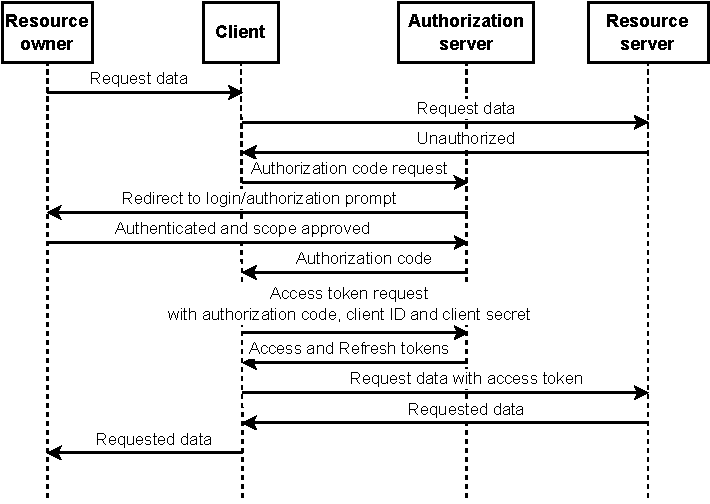
\includegraphics[width=.8 \linewidth]{figures/auth-sequence-auth-code.pdf}
  \caption{OAuth 2.0 Authorization Code Grant flow diagram}
  \label{fig:oauth2_auth_code_grant}
\end{figure}

\textbf{Authorization Code Grant} is a two-step process to obtain the access token. The user is first redirected to the authorization server with a request to obtain an authorization code. The authorization server authenticates the user and asks him for approval to grant the client specified scope of access to resources on the resource server. After the approval, the user is redirected back to the client with the authorization code. The client then uses the code together with client ID and client secret to make a request to the authorization server to obtain the access token. The authorization server then verifies the authorization code and issues the access token.

\subsection*{Proof Key for Code Exchange}
PKCE (Proof Key for Code Exchange) \cite{pkce_rfc} builds on top of Authorization Code Grant to further secure the process. It adds a secret called \emph{Code Verifier}. Code Verifier is then to transformed into a value called \emph{Code Challenge}, which is sent together with the authorization code request. Code Verifier is then sent together with the authorization code as a part of the access token request. The authorization server issues a new access token only if the received Code Verifier matches the one used to generate the Code challenge. This removes the risk of the authorization code being intercepted and used to generate the access token, as the authorization server will not create the access token without the Code Verifier, which is not part of the intercepted response.

\begin{figure}[hbt]
  \centering
  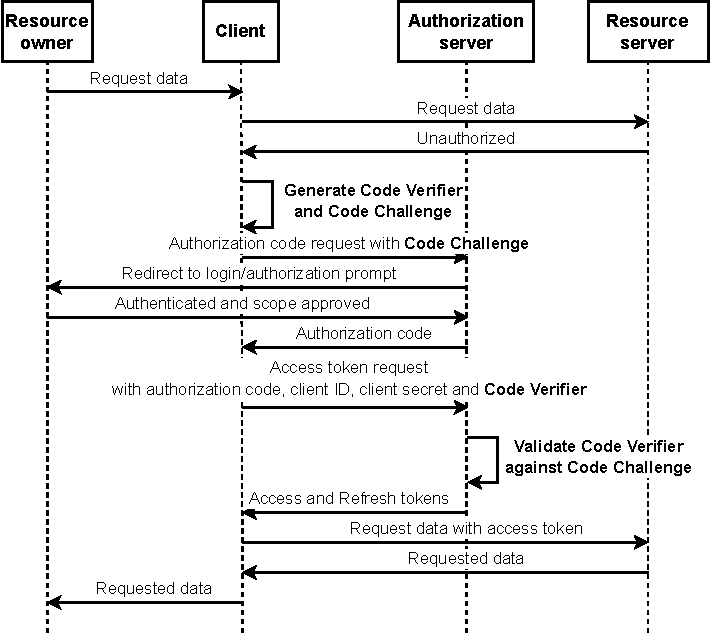
\includegraphics[width=.8 \linewidth]{figures/auth-sequence-pkce.pdf}
  \caption{OAuth 2.0 Proof Key for Code Exchange flow diagram}
  \label{fig:oauth2_pkce}
\end{figure}

\subsection*{Access and Refresh Tokens}
After successful authorization against the authorization server, the client is issued an \textbf{access token}. The client then uses this token to access the resources available on the resource server by sending it with each HTTP request in the Authorization header. Access tokens can be either an opaque string, called a \emph{bearer token}, or a \emph{sender-constrained token}. Sender-constrained tokens can be used only to authorize requests sent by the same client to whom the token was issued. This is usually achieved by asymmetric cryptography of the token. To comply with the standard, the token cannot convey user identity or any other information about the user.

Together with the access token, the authorization server also issues a \textbf{refresh token}, which can be used to generate a new access token without user interaction with the authorization server. This allows the authorization server to issue access tokens with a shorter expiration time, reducing the impact of the token being intercepted and stolen.

\subsection*{Scopes}
Compared to OAuth 1.0, OAuth 2.0 also introduces the concept of \emph{OAuth Scopes}, allowing the authorization server to issue access tokens with various limitations on access to resources. The scopes are defined by the resource server. The requested scope is part of the authorization request to the authorization server and is bound to the access token generated as a result of the authorization.

\subsection*{OpenID Connect}
OIDC (OpenID Connect) \cite{oidc} is an extension of OAuth 2.0, which allows the authentication of a user against the authorization server as well as obtaining basic user profile information about the authenticated user.

%=========================================================================

\chapter{Adaptor Design}
%\todo{Ref to OSLC spec}
%\todo{Gramar check}
%\todo{Style document}

This chapter deteails the process of designing the Jira and R4J adaptors, as well as the decisions made during the process and the reasoning behind them. The chapter is divided into several sections, each detailing different steps of the design process.

\section{Architecture Overview}
There are two possible ways, how to add the OSLC capabilities to a third-party web application -- either by extending the application via a plugin or by creating a separate self-contained application, that acts as a middle-man between the third-party application and the user. Both of these approaches can be used to create the adaptor for Jira and R4J, as Jira allows the creation of third-party plugins and it exposes its data thourh the REST API. At the start of the design process a decesion was made, to keep the adaptor as generic as possible, to allow the option to turn it into a generic adaptor for requirement management specification in the future. This would allow its use with other third-party requirement management applications by utilizing the strategy design pattern \cite{strategy_design_pattern}, to switch the data-access layer of the adaptor. With this in mind, the second approach, to create a standalone web application, was chosen, as there is no way to create a plugin, that would be compatible with every possible third-party application.

After careful consideration of the capabilities and data exposed by both Jira and R4J, it was determined, that the best option would be to split the adaptor into two separate adaptors, one for Jira and second for R4J. This is in line with the decesion to keep the adaptor as generic as possible. The Jira adaptor would be responsible for satisfying the requirements of the OSLC Core and Requirement Management Specification. The R4J adaptor would add some additional functionality provided by R4J, while not putting any restrictions, on what functionality has to be provided by any other third-party requirement management applications, in order to be compatible with the generic adaptor. These adaptors can then be used together to provide the full functionality, or users can opt to use only the Jira adaptor, if they do not need the additional functionality or if they do not have an active subscription to the R4J plugin, while still retaining the compliance with the OSLC Core and Requirement Management Specification.

\section{Tools Selection}
One of the initial steps of the desing process was the selection of the language, libraries and tooling, that would be used to implement the adaptors. At the time the design process started, there were only two real language options available for consideration, being \texttt{C\#} and Java. 

The OSLC4Net \cite{oslc4net} library for \texttt{C\#}, developed by the OSLC team, was in an unusable state at the time, as it has been overlooked and not maintained for a long time. It has recently started getting some attencion, at the time of writing this thesss, so if the library is brought up to date and additional tooling is developed, it might become a viable option in the future.

Because of the state of OSLC4Net, the only viable option left was to use Java with the well maintained OSLC4J SDK, together with the Eclipse Lyo tooling for developement of OSLC applications. The code generator included in Eclipse Lyo, generates the code skeletons for the adaptors as Eclipse Jetty servers \cite{jetty} equiped with Apache Maven \cite{maven} for dependency management and build automation.

\section{Adaptor Modeling}
After tooling selection, the next step in the design process, was to model the adaptors themself. The modeling was done using the Eclipse Lyo modeling tool, which also provides the ability to generate code skeletons from the created models. Most of the modeling process is based on the tutorials \cite{oslc_domain_workshop}\cite{oslc_toolchain_workshop}\cite{youtube_lyo_tutorial} and examples \cite{github_oslc_lyo-adaptor-sample-modelling}\cite{github_oslc_bugzilla} provided by the OSLC community, as well as adaptor models for Unite \cite{unite_gitlab}. The modeling of the adaptors can be separated into two steps, domain modeling -- modeling the resources accepted and exposed by the adaptor, and toolchain modeling -- modeling the functionality and capabilities of the adaptor, both of which are described in the following sections.

\subsection{Domain Modeling}
The domain models were created based on the OSLC Core and Requirement Management Specification, with the data exposed by Jira and R4J APIs taken into consideration. The main goal was to create models compliant with the standards, while taking into account their extensibility in the future and without creating any limitations by coupling them with Jira or R4J specific resources. This lead to the separation into \texttt{oslc}, \texttt{oslc\_rm}, \texttt{jira} and \texttt{jira\_r4j} namespaces. The \texttt{oslc} and \texttt{oslc\_rm} models were modelled using the models provided by Lyo project \cite{lyo_domains} as a base.

%todo: zmínit MUST, SHOULD ...

\subsection*{OSLC Core Domain}
The OSLC Core domain model is specified by the OSLC Core specification described in \ref{sec:oslc_core_specification}. As every OSCL compliant adaptor has to implement the OSLC Core specification, the domain model provides the base resources of the OSLC Core vocabulary as well as other basic namespaces used for the definition of other resources -- namely RDF, RDFS, Dublin Core and FOAF. %TODO: add citations

\todo{Add Core Domain diagram}

\subsection*{OSLC Requirement Management Domain}
The OSLC Requirement Management domain model defines the \texttt{oslc\_rm:Requirement} and \texttt{oslc\_rm:RequirementCollection} resources, based on the models from Lyo project. Properties, that are not required by the Requirement Management specification and are not needed in this thesis, have been removed and the representations have been extended by the properties defined in \texttt{jira} namespace.

\todo{Add Requirement Management diagram}

\subsection*{OSLC Jira and R4J Domains}
The \texttt{jira} and \texttt{jira\_r4j} namespaces define properties and resources, that represent resources and properties native to Jira and R4J. The \texttt{jira\r4j:Folder} has been defined in a way, where it references \texttt{oslc\_rm:Requirement} and \texttt{oslc\_rm:RequirementCollection}, instead of the other way around, to allow the use of the Jira adaptor independently of the R4J adaptor.

\todo{Add Jira and R4J Domain diagram}

\subsection{Toolchain Modeling}
% toolChain 
% diag

% Adaptor diags
% remove the person and project query from the diagram

\section{Mapping OSLC resources to Jira and R4J}
%kecy plky o tom jak to musí být generické protože každý Jiru používá jinak nebo nemá práva na to přidávat další fieldy
%GUID identifier - why + benefits
%\todo{Možnost uložení identifikátorů v labels fieldu}
%\todo{Identifikátory Requirement a RequirementCollection}
%\todo{req a reqCollection type name nesmí být stejné}
%\todo{Limitace + co dělat když nejde něco přidat do Jiry}
%problem with Epic as it requires EPIC name field as well - nevadí - zmínit že můžou existovat issue typy s jinými povinnými fields

%=========================================================================

\chapter{Implementation}
%\todo{Gramar check}
%\todo{Style document}

%\todo{Authentizace Basic + OAuth, not sure if here nebo v Adaptor Design zmínit jak to generuje Lyo a jak to používáme/bylo změno}
%\todo{Popis toho jaké jdou dělat query}
%\todo{Konfigurační soubory pro Jiru a R4J}
%\todo{permision needed for user to do CRUD operations}
%JIRA - JQL
%R4J local filtration - navrhnout suggestion missing endpointu (teoreticky možná optimalizace s cache přes timestamp a checkem jestli existuje issue s modified > než time stamp -> get again, not ideal ale lepší než nic, za předpokladu že modifed lookup by byl rychlejší)

%Popsat Oauth - OSLC není povínné řešit, přeposílání na Jira -> stará se o to ona

%Query jenom základ, neexistuje knihovna co by to řešila

%\todo{BUGv R4J API: 500 returned při updatu folderu s parent=ROOT}

%Memory leak caused by not closing connections - fixed by closing all opened in SessionDestroy

%=========================================================================

\chapter{Evaluation and Testing}
%\todo{Gramar check}
%\todo{Style document}

%\todo{Testování v Postmanovi}

%\todo{Testování pomocí ReqIF souboru}

%eval OSLC 
%zmínit složitost setupu Eclipse Lyo a zastaralé dokumentace k instalaci

%eval Req Spec

%eval JIRA + R4J API
%Hard to tell when 401 as Jira returns 400/404 as Anonymous access exists

%eval result
%\todo{Pokud požiju R4J hledám pomocí folder a získávám jenom Bugs/Reqs které jsou  nalinkované v R4J, pokud využitu JIRA adaptor získávám všechny issues daného typu (v configuraci) -> JIRA adaptor potřebuje speciální issues types aby rozlišoval mezi req a jinými issues}
%jira adaptor can function on its own

%future work
%možnost přidat OIDC nebo OAuth PKCE do budoucna

%=========================================================================

\chapter{Conclusion}
%\todo{Gramar check}
%\todo{Style document}


%=========================================================================

% For compilation piecewise (see projekt.tex), it is necessary to uncomment it
% \end{document}